\documentclass{scrartcl}
%\usepackage{draftwatermark}
%\SetWatermarkText{DRAFT}
%\SetWatermarkScale{5}

\usepackage[pdftex,dvipsnames]{xcolor}  % Coloured text etc.
\usepackage[utf8]{inputenc}
\usepackage{tikz}
\usepackage{graphicx}
\usepackage{amsmath}
\usepackage{amssymb}
\usepackage{hyperref}
\usepackage{algorithm2e}
\usepackage{placeins}
\usepackage{float}
\usepackage{xargs}     
\graphicspath{ {img/} }
% Use more than one optional parameter in a new commands
% 
\usepackage[colorinlistoftodos,prependcaption,textsize=tiny]{todonotes}
\newcommandx{\unsure}[2][1=]{\todo[linecolor=red,backgroundcolor=red!25,bordercolor=red,#1]{#2}}
\newcommandx{\change}[2][1=]{\todo[linecolor=blue,backgroundcolor=blue!25,bordercolor=blue,#1]{#2}}
\newcommandx{\info}[2][1=]{\todo[linecolor=OliveGreen,backgroundcolor=OliveGreen!25,bordercolor=OliveGreen,#1]{#2}}
\newcommandx{\improvement}[2][1=]{\todo[linecolor=Plum,backgroundcolor=Plum!25,bordercolor=Plum,#1]{#2}}
\newcommandx{\thiswillnotshow}[2][1=]{\todo[disable,#1]{#2}}

\title{COMSW4444 CC2 Report}
\author{
\textbf{Group 6}: Diana Liskovich, Parthiban Loganathan, Robert Ying}
\date{November 2015}

\restylefloat{table}
\usetikzlibrary{shapes,arrows,positioning,patterns}

\tikzstyle{decision} = [diamond, draw, fill=blue!20, 
    text width=8em, aspect=2, text badly centered, node distance=3cm, inner sep=0pt]
\tikzstyle{block} = [rectangle, draw, fill=blue!20, 
    text width=10em, text centered, rounded corners, minimum height=4em]
\tikzstyle{line} = [draw, -latex']
\tikzstyle{cloud} = [draw, ellipse,fill=red!20, node distance=3cm,
    minimum height=2em]

\begin{document}

\maketitle

\tableofcontents

\pagebreak

\section{Introduction} % DRI: Diana

\subsection{General goal}
We are presented with a 50 $\times$ 50 grid of dough. Two players compete at a time, each choosing three cutters. If the players choose the same shape, the shape is not valid, and they have to choose again. The three cutters are of size 11, 8, and 5. Each shape must be a valid undecomino, octomino, or pentomino, respectively---that is, each cell must share an edge with at least one other cell.

Once the shapes are chosen, the cutting of the dough begins. One player is chosen at random to make the first move, which must be the placement of a pentomino. Afterwards, the players alternate placing any piece in a valid location, e.g. one which does not include a cell which has already been cut in a prior tick.

The game ends when moves can no longer be made on the board. The winner is the player with a higher score, where the score is the number of cookies cut by each player.

\subsection{Basic idea}
There are two main considerations in creating a winning strategy. The strategy of piece selection and the strategy of piece placement. 

The piece selection strategy should incorporate a design for the case where the first choice shape is also chosen by the opponent. A consideration for the piece placement strategy is how destructive and how constructive it will be. 

Additionally, the strategies of competitors are important to consider. The effectiveness of our strategy may depend on which shapes and strategies are used by the opponent. It may be helpful to be dynamic in this case.

However, compute time is a limitation to this problem. How dynamic our strategies are and how extensive our searches are are constrained by this factor, as search trees of higher depth can perform better than first-order analyses. In order to attain our goal of conquering more of the board than our competitors it is important to consider these different aspects of the problem.

% end Introduction

\section{Problem Analysis} % DRI: Robert

\subsection{Fundamental analysis}
During the course of the in-class discussion, a fairly wide variety of strategies were proposed and experimented with. While we go more into a subset of these strategies in Sec.~\ref{sec:techniques}, we can break them into a few general categories.

The first strategies were strongly dependent on undecomino (11-cookie-cutter) selection, using variants of tessellated shapes or Matryoshka-esque nesting shapes to deny space to the opponent. These started with the general assumption that it would be better (in the constructive sense) to place undecominoes before octominoes before pentominoes, essentially front-weighting the number of cells acquired in each turn. During this stage in the game analysis, well-designed undecominoes were successful in locking down cookies for late-game placement.

The discussion then transitioned to strongly antagonistic strategies, intended to prevent the opponent from being able to place undecominoes later in the game. Some strategies used prior analytic approaches, e.g. axis-aligned bounding boxes with line-shaped pieces or placing pieces in the neighborhood of the opponent's last-placed piece. At first, we pursued these strategies using the same front-weighted piece ordering. Later, we discovered that it was often worthwhile to place smaller pieces in cases where there was a distinct comparative advantage, as can be seen in Fig.~\ref{fig:antagonistic_placement} below. Purely antagonistic strategies perform particularly well against purely constructive strategies, as the goal in the game is only to cut more cookies than the opponent.

Towards the end of the class discussions, more balanced strategies began to emerge, including some metagame-informed polyomino selection techniques. This was strongly detrimental to groups who had fairly brittle strategies---in particular, those using lines and axis-aligned bounding boxes.

From this process, we note that successful strategies must
\begin{itemize}
\item select polyominoes in reasonably optimal ways, e.g. lines, L-shapes, and diagonal-shapes.
\item be able to play low-rank polyominoes early in the game to block opponents
\item set up the board in the early game so as to increase piece placement opportunities in the late game
\item take advantage of as much information as possible at any given point, as limited by computational power
\end{itemize}

\subsection{Notes on the competition}
The development of competitive cookie-cutters has led to substantial trend-following between groups, as various groups discover techniques which are particularly effective in certain times and places. Group 6 is proud to note that we have been the originator of a number of these trends.

\begin{enumerate}
\item \textbf{Matryoshka strategies}: Simultaneously realized by groups 1, 4, 8, 9 in various forms early in the development process
\item \textbf{First-order move-scoring}: Initially used by groups 2 and 6, though eventually most teams ended up using some form of this method
\item \textbf{Antagonistic piece selection}: Used first by group 6 to select octominoes and pentominoes, and later generalized to help counter specific undecomino strategies
\end{enumerate}

As an early front-runner in the in-class discussions, we also noticed that many groups used group 6 as a testing benchmark. Eventually, many groups developed more complex strategies and move-scoring metrics by competing against group 6 and other groups with good overall performance.

% end Problem Analysis

\section{General Design} % DRI: Robert

% what we actually do
\subsection{Initial implementation}
\subsubsection{Polyomino selection}
Our initial strategy for selecting undecominoes assumed that the L-shaped undecomino was at least locally dominant, due to its ability to tessellate easily and thereby enclose space. We then selected the octomino and the pentomino as per Sec.~\ref{sec:selection}. During this stage of the discussion, most teams had fairly different undecomino selections, so we did not have a strategy for cases when we could not get our initial selection.

\subsubsection{Polyomino placement}
Our polyomino placement strategy is effectively to compute a score for each potential valid move in the game, and then pick the best move.

Selecting the set of valid moves is fairly straightforward: we can simply check the outer product of positions, shapes, and shape rotations to find which subset is playable. However, efficiently computing the score for each move is unfortunately more complex. As discussed in Sec.~\ref{sec:ourstrat}, we need to compute the number of potential enemy moves and the number of potential moves that we have at any given time, and then choose the one which has the best (lowest) score. However, computing the set of valid moves is fairly expensive, especially when evaluated over the $\approx 22,000$ moves available in the first few steps of the game.

Thus, we used a windowing method: the impact of a given move $m$ on the set of viable moves will only take effect within a 21 $\times$ 21 window surrounding the move, as the longest piece that can be placed is eleven cells long. Thus, it suffices to compute the change in the set of viable moves within these windows to find the best-scoring move in any given turn.

In the 50 $\times$ 50 game board, there are effectively $29^2$ windows to compute in each turn. We can precompute the pre-move scores of each window, and then compute the post-move score once per proposed move. As the computation of the number of viable moves is linear in the number of cells considered, this is a significant improvement, taking only $\approx 34$\%\footnote{$(29/50)^2$}of the time per potential move.

\subsection{Performance optimization}
\subsubsection{Polyomino selection}
See Sec.~\ref{sec:selection} and Sec.~\ref{sec:undecomino} for details. In short, we attempt to select a line-shaped undecomino, a diagonal-shaped undecomino, and an L-shaped undecomino in the initial stage, and then fit the octomino and the pentomino to the observed pieces. Our strategy is largely polyomino-agnostic, so the main goals are to select reasonable polyominoes while maximizing deficit to the opponent.

\subsubsection{Polyomino placement}
The total number of game moves in a given tick is a finite and relatively small number. Thus, we recreated our scoring algorithm using a form of memoization, where we store a lookup table mapping cells on the game board to the set of potential moves. This can be efficiently computed once per turn, but requires the creation of 2,500 \texttt{HashSet} objects.

Then, for each potential move, we need only take the union of the cells that the new move would overlap. This operation is still linear in the number of potential moves, but looks only at the moves which matter, eliminating from consideration the set of moves which are in the 21 $\times$ 21 window but not affected by the potential move. This significantly improved our overall runtime from $\approx 100$ seconds to $\approx 51$ seconds in each game, while returning the same move in each step as our earlier computation.

% end General Design

\section{Techniques}\label{sec:techniques}

% stuff we've tried or worked on

\subsection{Conditional polyomino selection}\label{sec:selection}

\subsubsection{Polyomino enumeration}
In this game, we use only pentominoes, octominoes, and undecominoes as potential cutter shapes, which are all shapes that can be described as polyominoes. A $k$-polyomino is made up of a set of $k$ squares, each of which shares at least one edge with another $k$-polyomino. Since we are allowed to rotate our polyominos arbitrarily, we need only consider polyominoes which are distinct under rotation, known as free polyominoes. This process lends itself well to a recursive algorithm to enumerate all valid polyominoes, which works roughly as follows:
\begin{enumerate}
\item Generate all $k$-polyominoes. The 1-polyomino is a single cell, which provides the base case.
\item For each adjacent unfilled cell, add the $k+1$th cell. This generates a list of $k+1$-polyominoes.
\item Filter the list of $k+1$-polyominoes to list only ``free'' polyominoes, e.g. removing rotations from the list
\item Repeat if the $k+1$-polyomino list is of insufficient rank, otherwise exit.
\end{enumerate}
As it turns out, there are only twelve free pentominoes and 369 free octominoes. Thus, it is actually quite practical to enumerate the full set of pentominoes and octominoes and store them inside of the Java source file for the submissions. This saves the requisite code complexity and runtime associated with enumerating each of the various polyominoes. Unfortunately, there are 17,073 undecominoes, so this is not quite as simple. As the undecomino is picked first, and only up to five unique undecominoes can be presented per team, it is generally unnecessary to enumerate the full set of undecomino pieces. Instead, we can choose a subset of five undecomino configurations which we know from the metagame analysis to be at least reasonably effective. We discuss these choices in Sec.~\ref{sec:undecomino}.

\subsubsection{Undecomino selection} % DRI: Parthi
The selection of undecomino is incredibly important and can determine which team dominates the game if we normalize for piece placement strategy. For example, it was observed in class that teams that selected straight line pieces generally dominated the game due to their ability to easily tile and fill in spaces within a small bounding box. We decided to use straight lines, diagonals and L-shape undecominos. To see why we chose this base set of undecominoes, see \ref{sec:undecomino}.

Our strategy is largely piece-agnositics and so we can play equally well regardless of which undecomino we choose. However, many opponent teams have strategies that are highly dependent on them picking a straight line undecomino. Our anti-line strategy in this case is to always pick the straight line ourselves. This either results in us getting the straight line or damaging the opponent by disallowing them from getting the straight line.

We then choose a diagonal piece as our second choice. This occurs if both players selected a straight line as their first choice. In such a case, most other teams pick a slight variant of the straight line, a hockey stick-like figure. This is countered by a diagonal which justifies selecting it as a second choice.

If both players selected a line as their first choice and a diagonal as their second choice, we resort to our original choice of L-shaped undecominoes since it is good at tiling and occupying space leading to early game dominance against long pieces that cannot break a matrix of Ls. Our final two choices are variants on the L-shape.

\subsubsection{Octomino and pentomino fitting} % DRI: Parthi
After selecting the undecomino, we have to choose the octomino and pentomino cookie cutters. These pieces are almost exclusively used in the end game. Given that most players are at most 1-2 pieces away from each other in score, being able to fill in the board with octomino or pentomino pieces at the end can determine the game. A strategic choice of these pieces based on our the opponent's as well as our own undecomino can drastically improve end game performance. In general, we choose octominos and pentominos that fit well with one of the larger pieces that have already been selected.

First, we need to describe how we evaluate a tiling piece to determine \textit{best fit}. Given a larger piece, we define the best fitting smaller piece as one which can make the most number of moves after the larger piece has made all possible moves on the board. It is a heuristic that broadly determines how well the selected piece fits in with the larger piece when these two are the only pieces under consideration.

For the octomino piece selection, we first attempt to choose the octomino which best fits our own undecomino. If it is unavailable, we then attempt to select a piece that best fits the opponent's undecomino. If both fail, we just go through the next best pieces that fit our own undecomino.

For the pentomino piece selection, we attempt to fit the opponent undecomino if our octomino succeeded in fitting our undecomino. If not, we fit our own undecomino. We pick the first such piece in decreasing order of fit.

\begin{figure}[h]
\centering
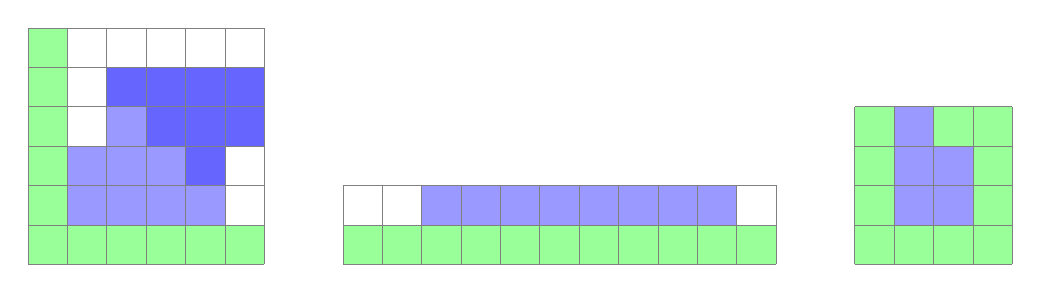
\begin{tikzpicture}
\fill[green!40!white] (0,0) rectangle (0.5,3);
\fill[green!40!white] (0,0) rectangle (3,0.5);

\fill[blue!40!white] (0.5, 0.5) rectangle (2.5, 1);
\fill[blue!40!white] (0.5, 0.9) rectangle (2, 1.5);
\fill[blue!40!white] (1, 1.4) rectangle (1.5, 2);

\fill[blue!60!white] (1, 2) rectangle (3, 2.5);
\fill[blue!60!white] (1.5, 1.5) rectangle (3, 2.1);
\fill[blue!60!white] (2, 1) rectangle (2.5, 1.6);
\draw[step=0.5cm,gray,very thin] (0, 0) grid (3, 3);

\fill[green!40!white] (4, 0) rectangle (9.5, 0.5);
\fill[blue!40!white] (5, 0.5) rectangle (9, 1);
\draw[step=0.5cm,gray,very thin] (3.999, 0) grid (9.5, 1);

\fill[blue!40!white] (10.5, 0) rectangle (12.5, 2);
\fill[green!40!white] (10.5, 0) rectangle (12.5, 0.5);
\fill[green!40!white] (10.5, 0) rectangle (11, 2);
\fill[green!40!white] (12, 0) rectangle (12.5, 2);
\fill[green!40!white] (11.5, 1.5) rectangle (12.1, 2);
\draw[step=0.5cm,gray,very thin] (10.499, 0) grid (12.5, 2);
\end{tikzpicture}
\caption{An assortment of undecominoes (green) and octominoes or pentominoes (blue) which fit closely to the chosen undecomino. From left to right, an L-shaped undecomino, a line-shaped undecomino, and a Matryoshka undecomino.}\label{fig:fitting}
\end{figure}

\subsubsection{Antagonistic polyomino selection}\label{sec:antagonisticselect}
There are a number of ways to aggressively use the polyomino selection process to gain an advantage in the game, though these are often dependent on a non-generalist strategy on the part of the opponent. We focus in particular on line-blocking and Matryoshka prevention.

\begin{itemize}
\item \textbf{Line-blocking}: Against most simple strategies, applying axis-aligned bounding box-based techniques to place straight-line polyominoes is particularly successful. However, these strategies become considerably less effective when placing a single polyomino does not also make a space to place another polyomino in the near future (as is true for line polyominoes). Thus, since our strategy is by-and-large polyomino agnostic, we choose a line as our first undecomino choice solely to prevent the opponent from being able to select this polyomino.

\item \textbf{Matryoshka prevention}: As discussed in Sec.~\ref{sec:matryoshka}, the pentomino or octomino necessary to complete the Matryoshka pattern is well-defined once the undecomino has been chosen. It is therefore practical to use a polyomino fitting algorithm to determine what piece this is, and then select it to prevent the opponent from successfully executing their strategy.

\end{itemize}

However, using a polyomino for antagonistic polyomino selection has a fairly significant cost. That is, there is a nontrivial chance that the player attempting antagonistic selection will end up taking the octomino or pentomino that was initially intended just to block the opponent. Thus, we must select whether to fit our octomino and pentomino to our own undecomino or our opponent's by analyzing the metagame.

From our empirical testing against all of the submissions during group discussion, it seems clear that either the octomino should fit the opponent and the pentomino ourselves, or vice-versa. This is not particularly surprising, as almost all games require a tradeoff between constructive and destructive behavior---fitting both the octomino and the pentomino to the opponent or oneself implies strong assumptions about piece placement which are often untrue in practice, e.g. local dominance or passive opponents.


\subsection{Polyomino-specific piece placement}

\subsubsection{Tessellation}

\begin{figure}[h]
\centering
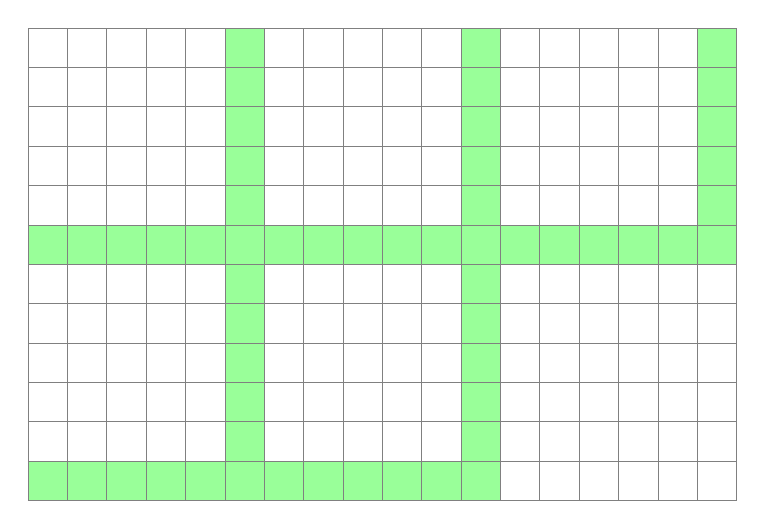
\begin{tikzpicture}

\fill[green!40!white] (2.5,0) rectangle (3,3);
\fill[green!40!white] (0,0) rectangle (3,0.5);

\fill[green!40!white] (2.5,3) rectangle (3,6);
\fill[green!40!white] (0,3) rectangle (3,3.5);

\fill[green!40!white] (5.5,0) rectangle (6,3);
\fill[green!40!white] (3,0) rectangle (6,0.5);

\fill[green!40!white] (5.5,3) rectangle (6,6);
\fill[green!40!white] (3,3) rectangle (6,3.5);

\fill[green!40!white] (8.5,3) rectangle (9,6);
\fill[green!40!white] (6,3) rectangle (9,3.5);

\draw[step=0.5cm,gray,very thin] (0, 0) grid (9, 6);

\end{tikzpicture}
\caption{An example of a tiling or tessellation-based strategy executed by the green player, designed to enclose the available space and thereby deny those cells to the opponent---a polyomino with a maximum side length of more than five cannot play in the above board.}\label{fig:tessel1}
\end{figure}

We initially decided to focus on a tiling strategy as a first attempt. Our initial algorithm used variants of L-shape cookie cutters which were tiled across the board. The intuition behind this was that tiling was both constructive and destructive. It was constructive in the sense that it covered a wide expanse of the board fairly quickly setting up board dominance in the early game if executed properly. It was destructive because it could potentially block opponent from placing their larger undecominoes forcing them to play the lower value octominoes earlier in the game. To achieve an effective balance of constructive and destructive play, such tiling has to be done strategically based on the opponent's cookie cutter such that the gap between our cuts is small enough to block the opponent's undecomino but is simultaneously structured in such a way that we can stack our own undecomino adjacent to the existing placements easily.

An example of tessellation using an L-shaped undecomino is visible in Fig.~\ref{fig:tessel1}. We can see that this is very good and preventing comparatively oblong polyominoes from being played at all, while maximizing board control early on in the game.

We decided to abandon this approach in favor of a polyomino-agnostic strategy since the success of this strategy relied heavily on good piece selection. However, as tessellation is an emergent behavior in many cases of piece-agnostic strategies, it is perhaps more correct to say that we generalize the logic behind tessellation during the actual polyomino placement process.

\subsubsection{Matryoshka placement}\label{sec:matryoshka}
This strategy is named after the Matryoshka nesting dolls, and was exhibited in the early stages of development by a number of groups. The basic idea of this strategy is to choose an undecomino which can partially enclose or interlock with the octomino or the pentomino selection.

\begin{figure}[h]
\centering
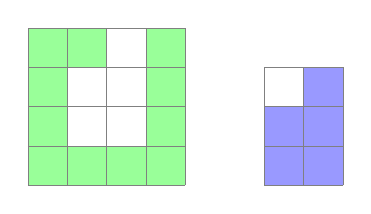
\begin{tikzpicture}
\fill[green!40!white] (0,0) rectangle (0.5,2);
\fill[green!40!white] (0,0) rectangle (2,0.5);
\fill[green!40!white] (1.5,0) rectangle (2,2);
\fill[green!40!white] (0.5,1.5) rectangle (1,2);
\draw[step=0.5cm,gray,very thin] (0, 0) grid (2, 2);

\fill[blue!40!white] (3,0) rectangle (3.6,1);
\fill[blue!40!white] (3.5,0) rectangle (4,1.5);
\draw[step=0.5cm,gray,very thin] (2.999, 0) grid (4, 1.5);
\end{tikzpicture}
\caption{A potential choice of an undecomino (green) and corresponding pentomino (blue) for the Matryoshka strategy.}\label{fig:matryoshka1}
\end{figure}

In Fig.~\ref{fig:matryoshka1}, the undecomino and pentomino nest perfectly into a 4 $\times$ 4 square, consuming a total of sixteen cells. The Matryoshka strategy is to place the undecomino pieces such that only the pentomino can be placed within it, guaranteeing the full sixteen cells per undecomino-placement (as opposed to eleven). At the end of the game, the pentominoes can then be filled in one-by-one. With these pieces, one way of pursuing this strategy is to place the undecominoes can be seen in Fig.~\ref{fig:matryoshka2}.

\begin{figure}[h]
\centering
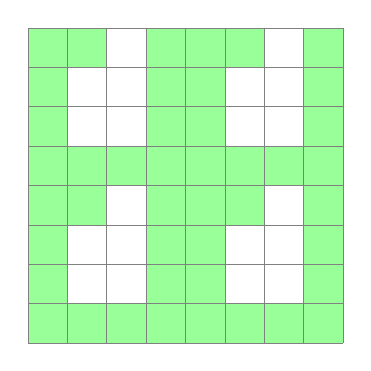
\begin{tikzpicture}
\fill[green!40!white] (0,0) rectangle (0.5,2);
\fill[green!40!white] (0,0) rectangle (2,0.5);
\fill[green!40!white] (1.5,0) rectangle (2,2);
\fill[green!40!white] (0.5,1.5) rectangle (1,2);

\fill[green!40!white] (0,2) rectangle (0.5,4);
\fill[green!40!white] (0,2) rectangle (2,2.5);
\fill[green!40!white] (1.5,2) rectangle (2,4);
\fill[green!40!white] (0.5,3.5) rectangle (1,4);

\fill[green!40!white] (2,0) rectangle (2.5,2);
\fill[green!40!white] (2,0) rectangle (4,0.5);
\fill[green!40!white] (3.5,0) rectangle (4,2);
\fill[green!40!white] (2.5,1.5) rectangle (3,2);

\fill[green!40!white] (2,2) rectangle (2.5,4);
\fill[green!40!white] (2,2) rectangle (4,2.5);
\fill[green!40!white] (3.5,2) rectangle (4,4);
\fill[green!40!white] (2.5,3.5) rectangle (3,4);

\draw[step=0.5cm,gray,very thin] (0, 0) grid (4, 4);
\end{tikzpicture}
\caption{Undecomino placement for the Matryoshka strategy}\label{fig:matryoshka2}
\end{figure}

Since the one open cell on the edge of the undecomino can be blocked off by placing the undecomino immediately below either a wall or another occupied cell, this strategy appears to be reasonable effective at first glance---certainly, it is difficult for an opponent to directly interfere with the piece placement process.

If we assume the opposing player to play purely constructively, the Matryoshka strategy results in a very small amount of unclaimed space on the board: the 2,500 cells can be largely covered by the Matryoshka-esque 4 $\times$ 4 blocks. For example, if both players are using similar Matryoshka strategies, they will be able to neatly divide the space into $\approx 1,200$ cells each, which is considerably more than in most strategies.

However, it is comparatively easy to counter a Matryoshka strategy at both the polyomino-selection and the polyomino-placement stages of the game. Firstly, the choice of undecomino uniquely determines the best pentomino for the Matryoshka strategy. Unfortunately, this is also available to the opposing team, so it is easy for the opposing team to choose the same pentomino or octomino and thereby prevent the Matryoshka player from executing the strategy effectively. Secondly, as the undecomino occupies only a 4 $\times$ 4 footprint, and as its axis-aligned bounding box closely resembles its actual shape, it is comparatively difficult for the Matryoshka-pieces to overcome highly antagonistic strategies, i.e. those which compute the axis-aligned bounding box of the undecomino and space themselves such that no undecominoes can be played.

\subsubsection{Placing lines with axis-aligned bounding boxes} % DRI: Parthi
For each shape, we can define a bounding box with the minimum height and width to contain it. Straight lines have the advantage of being able to fit in a single column or row. They have a very small bounding box profile. Suppose the width of the bounding box in the direction the opponent is attempting to tile them is $w$. To disrupt the tiling of opponent undecominoes, straight lines can be placed $w-1$ apart. This hurts the opponent but still allows us to place our straight line pieces at any one of the $w-2$ places between the two straight lines we just placed. Note the the opponent can possibly still use their octominoes or pentominoes in this space. However, if they do, we've succeeded in forcing them to play smaller pieces.

\begin{figure}[h]
\centering
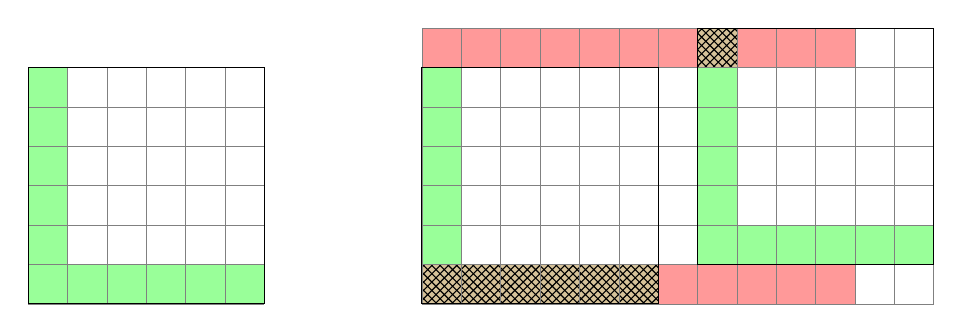
\begin{tikzpicture}
\fill[green!40!white] (0,0) rectangle (0.5,3);
\fill[green!40!white] (0,0) rectangle (3,0.5);
\draw[step=0.5cm,gray,very thin] (0, 0) grid (3, 3);
\draw[black, thin] (0, 0) rectangle (3, 3);

\fill[red!40!white] (5, 0) rectangle (10.5, 0.5);
\fill[red!40!white] (5, 3) rectangle (10.5, 3.5);

\fill[green!40!white] (5,0.5) rectangle (5.5,3);
\fill[green!40!red!40!white] (5,0) rectangle (8,0.5);
\fill[pattern=crosshatch, pattern color=black] (5,0) rectangle (8,0.5);

\fill[green!40!white] (8.5,1) rectangle (9,3.5);
\fill[green!40!red!40!white] (8.5,3) rectangle (9,3.5);
\fill[green!40!white] (8.5,0.5) rectangle (11.5,1);
\fill[pattern=crosshatch, pattern color=black] (8.5,3) rectangle (9,3.5);

\draw[step=0.5cm,gray,very thin] (4.999, 0) grid (11.5, 3.5);
\draw[black,thin] (5, 0) rectangle (8, 3);
\draw[black,thin] (8.5, 0.5) rectangle (11.5, 3.5);

\end{tikzpicture}
\caption{Here, the red player has placed a line-shaped undecomino exactly five spaces away from another line-shaped undecomino, which prevents the green player from playing the L-shaped undecomino in between, as signified by the cross-hatched overlapping cells.}\label{fig:aabb1}
\end{figure}

\subsection{Polyomino-agnostic piece placement}\label{sec:agnostic}

\subsubsection{Antagonistic placement} % DRI: Parthi
The goal of the game is to achieve a higher score than the opponent. Hence it is not sufficient to simply maximize our score. We also need to actively attempt to decrease the opponent's score.

An antagonistic or destructive strategy aims at minimizing the score of the opponent at any cost. One such strategy employed by some teams is aggressive "following" where the player placer its piece next to the opponents to block the opponent from tiling. Pieces are placed to either minimize the number of moves the opponent can play or to force the opponent to play smaller pieces with the overall goal of preventing them from increasing their score.

In a purely antagonistic strategy, it is acceptable to make suboptimal moves in order to hurt the opponent. For example, the player might use an pentomino even when an undecomino can be placed in order to prevent an opponent from placing an undecomino. It is also possible that we make moves that prevent both the opponent and ourselves from placing a piece.

We shall formalize in this in our piece placement strategy as described in Sec.~\ref{sec:ourstrat}.

\begin{figure}[h]
\centering
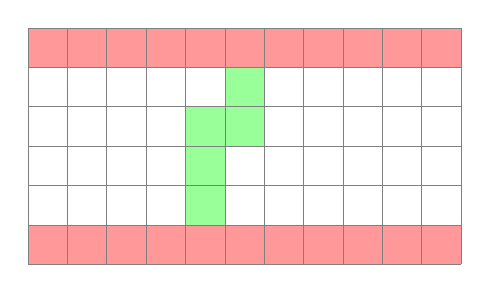
\begin{tikzpicture}
\fill[red!40!white] (0,0) rectangle (5.5,0.5);
\fill[red!40!white] (0,2.5) rectangle (5.5,3);

\fill[green!40!white] (2,0.5) rectangle (2.5,2);
\fill[green!40!white] (2.5,1.5) rectangle (3,2.5);

% \fill[green!40!white] (5,0.5) rectangle (5.5,3);
% \fill[green!40!red!40!white] (5,0) rectangle (8,0.5);
% \fill[pattern=crosshatch, pattern color=black] (5,0) rectangle (8,0.5);

\draw[step=0.5cm,gray,very thin] (0,0) grid (5.5,3);

\end{tikzpicture}
\caption{Here, a pentomino is placed by the green player to prevent the red player from placing a set of line-shaped undecominoes.}\label{fig:antagonistic_placement}
\end{figure}

\subsubsection{Constructive placement} % DRI: Parthi
In order to maximize our own score, the player needs to command the board by placing larger pieces earlier and capturing areas of the board where we can play smaller pieces in the end game that the enemy can't touch. To implement this, we need some metric or score to decide which move to choose. We formalize this in Sec.~\ref{sec:ourstrat} below. 

\subsubsection{Our strategy: Formalizing constructive and destructive placement}\label{sec:ourstrat} % DRI: Parthi
In our final strategy, we determine which move to play based on a score function we define as below:

\begin{equation}
s = \sum_{m} \text{WNBLOCK}_{\text{self}}\left(m, \frac{1}{2}\right) - \text{WNBLOCK}_{\text{opponent}}(m,1) - |m|
\end{equation}
where $m$ is a move under consideration, $|m|$ is the size of the shape placed in move $m$, and WNBLOCK is defined as
\begin{equation}
\text{WNBLOCK}_{k}(m,p) = \sum_{m \in \text{BLOCKED}_k} |m|^p
\end{equation}
and BLOCKED represents the set of moves blocked by $m$.

Our goal is to minimize the score $s$ so we compute the score of all possible valid moves we can play and pick the minimum. This leads to a number of emergent behaviors:
\begin{itemize}
\item Blocking enemy moves is more important than avoiding blocking our own moves
\item If all else is equal, we play larger (greater $|m|$) moves first
\item Moves which the enemy cannot block (e.g. the enemy cannot place a piece that the move blocks) are generally played after moves which the enemy can block
\end{itemize}

We chose the values of $\frac{1}{2}$ and $1$ for the $p$ above by testing a variety of potential scoring functions. After the last class submission, we noted that this score function (along with our general strategy) was able to successfully defeat all of the other groups. Unfortunately, between the last class submission and the final tournament submission, it appears that a number of other groups have drastically changed their strategies, so this score function is probably no longer optimal.

Computing such a score from scratch on each turn of the game is computationally infeasible. In our implementation, we create a hash table that maps each point $(i,j)$ on the board to the set of all possible moves that would contribute to the score by cutting the dough at the point $(i,j)$. We create a similar hash table for enemy moves as well.

On each turn, we need to iterate through all valid moves we can make and then compute the score function $s$ using these two hash tables to compute the number of blocked moves and number of blocked enemy moves.

\begin{figure}
\centering
\includegraphics[width=0.85\textwidth]{img/nummoves}
\caption{Number of moves we evaluate on each turn}
\label{fig:nummoves}
\end{figure}

Note that the actual implementation also essentially ignores moves that do not block any enemy moves by increasing score by $10^6$. This ensures that we do not attempt to place pieces in areas where we have command of the board, since we are guaranteed to be able to put a piece there later without any risk of the opponent stealing that area.

\subsubsection{Minimax analysis} % DRI: Parthi
The cookie cutter game is a competitive two player game that lends itself well to minimax, a game playing strategy used to minimize the loss in a worst case scenario. Such a strategy is common in games like chess or Othello. We use an exhaustive tree based search on multiple game states to a certain depth. The problem with a minimax approach is that there are so many possible moves early on in the game that using it leads to an impractically long runtime. To take advantage of this strategy, we wait to use perform the minimax search till the end of the game where there is a limited number of valid moves left. The constrained search space makes the problem tractable and can improve end game move selection.

\begin{figure}
\centering
\includegraphics[width=0.7\textwidth]{img/minimax}
\caption{An example of minimax to depth 4}
\label{fig:minimax}
\end{figure}

In our implementation, we attempted to search to a depth of 4 when there were less than 200 valid moves left in the game. These parameters were not optimal. We did not include minimax in the final submission since it increased runtime without improving performance. We suspect that given time, we could have fine-tuned our parameters, come up with a better choice of score function and implemented optimizations to store game state more efficiently.

Refer to code\footnote{\url{https://github.com/rbtying/comsw4444-cc2/blob/lookahead/Player.java\#L226}} for details.

% end Techniques

\section{Empirical Testing and Results} % DRI: Diana

\subsection{Empirical Testing}
Throughout the course of the class discussion and the development of our own strategy, we spent a significant amount of time testing various strategies against one another. This was particularly important in this project because there is no simple intuition as to which techniques are the most effective, e.g. the constructive vs antagonistic placement tradeoff, the choice of initial pieces, and the like. In particular, the effectiveness of various strategies is strongly dependent on the opposing player---nearly every strategy has its own particular strengths and weaknesses. In the preceding sections, we have noted some of our findings with respect to these tradeoffs, and how they impact the flow of the cookie-cutting process.

As an initial breakdown, we tested the two stages of the game separately, evaluating various polyomino-selection strategies independent of polyomino-placement strategies and vice-versa. This is a somewhat safe assumption, as we note that most polyomino-specific placement strategies can be found as emergent behaviors as a result of sufficiently complex polyomino-agnostic placement strategies, as noted in Sec.~\ref{sec:agnostic}.

\subsubsection{Choice of undecomino}\label{sec:undecomino}
In the polyomino-selection stage, we found that the most important factor was the selection of the undecomino, as the octomino and pentomino could take advantage of in-game knowledge of the opponent's undecomino selection. In contrast, the undecomino selection is dependent solely on meta-strategic notes from in-class discussion and empirical testing.

The process we used to evaluate the various undecomino choices was to run a series of games using our most recent polyomino placement algorithm. This was considered to be a good heuristic because our strategies consistently performed well in the in-class discussions. Of course, our own strategy piece placement strategy was certainly not the best out of those implemented in class, so our choice of undecomino may be overfitted to our piece placement algorithm.

\begin{figure}[h]
\centering
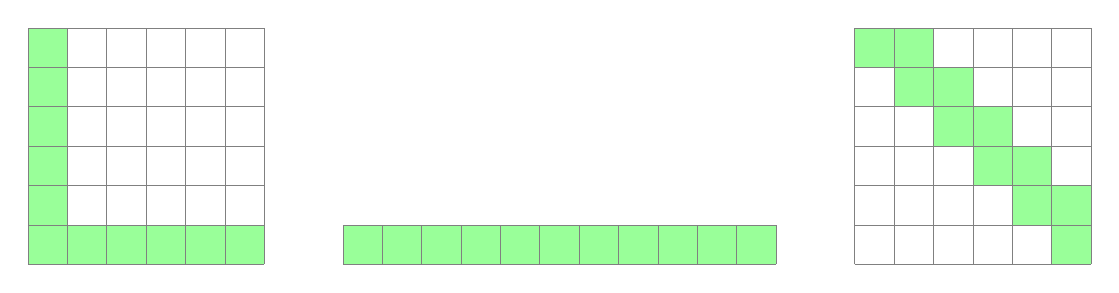
\begin{tikzpicture}
\fill[green!40!white] (0,0) rectangle (0.5,3);
\fill[green!40!white] (0,0) rectangle (3,0.5);
\draw[step=0.5cm,gray,very thin] (0, 0) grid (3, 3);

\fill[green!40!white] (4, 0) rectangle (9.5, 0.5);
\draw[step=0.5cm,gray,very thin] (3.999, 0) grid (9.5, 0.5);

\fill[green!40!white] (10.5, 2.5) rectangle (11.5, 3);
\fill[green!40!white] (11, 2) rectangle (12, 2.5);
\fill[green!40!white] (11.5, 1.5) rectangle (12.5, 2);
\fill[green!40!white] (12, 1) rectangle (13, 1.5);
\fill[green!40!white] (12.5, 0.5) rectangle (13.5, 1);
\fill[green!40!white] (13, 0) rectangle (13.5, 0.5);
\draw[step=0.5cm,gray,very thin] (10.499, 0) grid (13.5, 3);

\end{tikzpicture}
\caption{An assortment of initial undecomino choices. From left to right: an L-shaped undecomino, a line-shaped undecomino, and a squiggle-shaped undecomino.}\label{fig:undecomino_selection}
\end{figure}

\subsubsection{Move scoring}
As discussed in Sec.\ref{sec:ourstrat}.

\subsection{Tournament results}

Overall, we dominated five groups \{g1, g4, g5, g8, g9\} and in turn consistently lost to 3 groups \{g2, g3 and g7\}. Group 3 uses a minimax strategy that could have made the difference in winning the tournament. Group 2 also uses lines and diagonals, which forces us to use L-shaped undecominoes.

In total, we win 47 out of 80 games. In terms of total wins, g3 wins 76, g7 wins 70 and g5 wins 50 putting us in fourth place.

The results are expected given that groups 3, 6 and 7 were top performers early on in the project with our group quickly becoming a target to beat.

\begin{table}[h]
\centering
\caption{Group 6's win/loss record against the other 8 groups. We found that this record was independent of which group was playing the first move.}
\begin{tabular}{|c|c|c|}\hline
Group & Wins & Losses \\ \hline
g1 & 10 & 0 \\ \hline
g2 & 0 & 10 \\ \hline
g3 & 0 & 10 \\ \hline
g4 & 6 & 4 \\ \hline
g5 & 10 & 0 \\ \hline
g7 & 1 & 9 \\ \hline
g8 & 10 & 0 \\ \hline
g9 & 10 & 0 \\ \hline
\end{tabular}
\label{tab:tournament1}
\end{table}

\begin{table}[h]
\centering
\caption{Each group wins more than half the games against at least one other group. This table lists the groups that a given group consistently wins against.}
\begin{tabular}{|c|l|}\hline
Group & Dominated Groups \\ \hline
g3 & g1, g2, g4, g5, g6, g7, g8, g9 \\ \hline
g7 & g1, g2, g4, g5, g6, g8, g9 \\ \hline
g2 & g1, g4, g6, g7, g8 \\ \hline
g6 & g1, g4, g5, g8, g9 \\ \hline
g5 & g1, g2, g4, g8, g9 \\ \hline
g8 & g1, g4, g9 \\ \hline
g4 & g1, g9 \\ \hline
g9 & g2 \\ \hline
g1 & g9 \\ \hline
\end{tabular}
\label{tab:tournament2}
\end{table}

\begin{table}[H]
\centering
\caption{This table lists the mean and standard deviation of group scores in each matchup.}
\label{tab:tournament3}

\begin{tabular}{|c|c|c|c|} \hline
Group & Group 6 Score & Opponent Score & Score Delta \\ \hline
g1 & $1139.2 \pm 26.4$ & $895.4 \pm 10.8$ & $243.8 \pm 30.3$ \\ \hline
g2 & $1009.5 \pm 13.1$ & $1076.6 \pm 13.0$ & $-67.1 \pm 24.7$ \\ \hline
g3 & $888.3 \pm 30.1$ & $1056.4 \pm 17.1$ & $-168.1 \pm 46.1$ \\ \hline
g4 & $1114.3 \pm 53.7$ & $1085.6 \pm 72.4$ & $28.7 \pm 85.5$ \\ \hline
g5 & $1095.2 \pm 19.9$ & $995.6 \pm 9.4$ & $99.6 \pm 28.5$ \\ \hline
g7 & $911.2 \pm 14.3$ & $963.9 \pm 20.1$ & $-52.7 \pm 29.4$ \\ \hline
g8 & $1055.7 \pm 22.1$ & $941.7 \pm 12.3$ & $114.0 \pm 27.9$ \\ \hline
g9 & $1103.2 \pm 21.0$ & $901.0 \pm 15.3$ & $202.2 \pm 30.0$ \\ \hline
\end{tabular}
\end{table}

\subsubsection{Overall Analysis}

Given the scores of competing teams, there are several ways to assess performance. The total number of wins that each group had are visualized below. As mentioned, our group, g6, received fourth place for that measure.

\begin{figure}[H]
  \includegraphics[width=\linewidth]{numberOfWins.png}
\end{figure}

In order to compare the degree of dominance of one strategy over another, it is useful to consider the number of points by which the winning team won. For example, a strategy where the difference between the scores of the teams is the placement of one piece, is different from a situation where dominance is by ten pieces. We computed the average number of points by which each strategy dominated for winning games. We have the second highest score in this category. This means that for the games which we won, we had won by a greater margin than most other teams. This suggests that our strategy was stronger in beating the opponents that we dominated, as discussed above.  

\begin{figure}[H]
\includegraphics[width=\linewidth]{marginOfWinning.png}
\end{figure}

Similarly to the measure above, we measured the margin of loss averaged over all the games in which a team lost. The goal is to identify whether there is a strong or weak dominance of one strategy over the ones it dominates. We have the third lowest score for this measure. This means that on average when we lost a game, we didn't lose with as much of a margin as other teams did. 

\begin{figure}[H]
\includegraphics[width=\linewidth]{MargOFLosing.png}
\end{figure}

The above figures suggest that even though we didn't have the most number of wins, when we lost to other teams, we did not lose by a strong margin, and when we beat other teams, we won by a large margin. Even though we did not have the greatest number of wins, this shows that we had a strong strategy.

This idea can be broken down further by adding weights to the dominance graph we computed. We can see by how many points each team dominates another team on average. 

\begin{table}[H]
\centering
\begin{tabular}{|c|l|}\hline
Group & Dominated Groups = Avg. Loss \\ \hline
g3 & g1=403, g2=91, g4=297, g5=185, g6=161, g7=66, g8=342, g9=343 \\ \hline
g7 & g1=74, g2=155, g4=105, g5=23, g6=60, g8=107, g9=91 \\ \hline
g2 & g1=284, g4=71, g6=67, g8=112 \\ \hline
g6 & g1=244, g4=89, g5=100, g8=114, g9=202 \\ \hline
g5 & g1=151, g2=124.5, g4=160, g8=86, g9=93 \\ \hline
g8 & g1=29, g4=27, g9=25 \\ \hline
g4 & g1=269, g9=23 \\ \hline
g9 & g2=93 \\ \hline
g1 & g9=107 \\ \hline
\end{tabular}
\end{table}


% end Empirical Testing and Results

\section{Conclusions and future work} % DRI: Diana, Parthi
Our strategy ended up doing fairly well in the competition. It was important to minimize the moves of our players while maximizing our potential - both in shape selection and placement. The results of the game demonstrate that there was no one clear winner or dominating team. Each strategy had its strengths and failures, which were made vulnerable or not based on the opponent the team was playing. The complexity of the strategies was magnified by the fact that there was the shape selection and placement to consider. Overall, the problem had many interesting aspects to analyze, experiment with, and optimize. Had we had even more time, we could have implemented even further tactics and complexity.

Here are some directions in which we could take this project:

\begin{enumerate}
\item Most teams used one of a few select pieces such as lines, diagonals or in our case L-shapes. As we showed in our polyomino enumeration, there are numerous other pieces that might result in interesting behavior. One strategy briefly discussed in class was to create predefined sets of undecomino, octomino and pentomino pieces that perform well together and to define sets that exhibit dominant behavior over other sets. Then piece selection is a matter of searching through these sets. This would give us a wider variety of pieces to pick from.
\item Our minimax strategy could have been successfully included in the final submission if we had tuned our parameters and architected our code such that we could save game state without a major refactor. The minimax strategy also operates under the assumption that the opponent is rational and makes the same move choice as ourselves given the chance. This is clearly not the case and a move selection adapted to each team could have been used.
\item We could have potentially limited our piece placement search strategy to predict optimal moves locally, rather than globally on the board. This may have ended up hurting our margin of success or failure, but it is something that could be experimented with even further. Saving some computation time for these searches could allow us to use up more CPU time resources on other computations.
\item Given that this game relies a great deal on opposing strategies, we could have added some kind of deception tactic to our game. Knowing what common heuristics are used to decide on a next move for our opponents, those can be sabotaged, just as we tried to sabotage shape selection for our opponents.
\end{enumerate}

% end Conclusions

\section{Acknowledgments} % DRI: 

We would like to thank Professor Ross and the rest of the class for valuable and stimulating class discussions. We would also like to thank George and Orestis for providing the class with a simulator and skeleton on which to develop our strategy and for conducting the tournament. A lot of our developments came from improvements made to the simulator, conversations brought up in class discussions, and having the opportunity to watch teams perform under different circumstances and states in class.  

% end Acknowledgements

\FloatBarrier

\appendix

\section{Summary of contributions} % DRI: All

\begin{table}[h]
    \centering
    \caption{Summary of contributions}
    \begin{tabular}{|r|l|} \hline
                                          & Windowed move evaluator; \\
        \textbf{Robert Ying}              & Anti-line strategies; \\
                                          & Piece-fitting algorithm; \\ \hline
                                          & Minimax strategy; \\
        \textbf{Parthiban Loganathan}     & Undecomino selection; \\
                                          & Competitor analysis; \\ \hline
        \textbf{Diana Liskovich}          & CPU time minimization strategies and experimentation; \\
                                          & Game analysis; \\ \hline
    \end{tabular}\label{tbl:contrib}
\end{table}


\end{document}
